\par Dans la présente Section, on va découvrir ce qui a été concrètement réaliser durant le stage, ainsi que tout les outils utilisés pour mener a bien les différents projets. J'essayerais, par la suite, de présenter un bilan général des six mois de stage.  

\begingroup
    \let\clearpage\relax
    \chapter{Environnement technique et outils technologiques}
\endgroup
\section{Outils communs}
\par Dans la présente section, je présenterais tout les outils commun a tout les projets, notamment les outils fonctionnels (outils de planification \dots) ainsi que les outils pour vérifier la qualité du code et déploiement des applications. 
\subsection{La suite Atlassian}
\par Atlassian est un éditeur de logiciels, basé en Australie, qui développe des produits pour la gestion de développement et de projets. Ses logiciels les plus connus sont Jira, Confluence, Bamboo, Bitbucket et Trello. Une grande parte de la suite Atlassian est payante.
\par Pour nos projets, j'ai pu utiliser JIRA et Confluence.

\subsubsection{Jira}
\par JIRA est un « issue tracker ». On pourrait traduire : un « Gestionnaire de demande ». Cette définition donne une idée du potentiel de l’outil mais reste néanmoins imparfaite parce que le terme anglais « Issue » fait référence à quelque chose de beaucoup plus générique. Une « Issue » est en fait un objet, sujet, ou situation, susceptible d’être traité. Il peut donc s’agir de bug, d’anomalies, d’incidents, de demandes d’intervention, mais aussi de la multitude des taches anodines qui font le quotidien de chacun d’entre nous. JIRA est un outil de suivi d’activités.
\clearpage
\par En pratique les cas d’utilisation de JIRA les plus souvent rencontrés sont les suivants :
\begin{itemize}
    \item La gestion du support et des activités de développement logiciel
    \item Le suivi des anomalies
    \item Le suivi d’activité
    \item La gestion de Centres de services
\end{itemize}
\begin{figure}[ht]
    \centering
    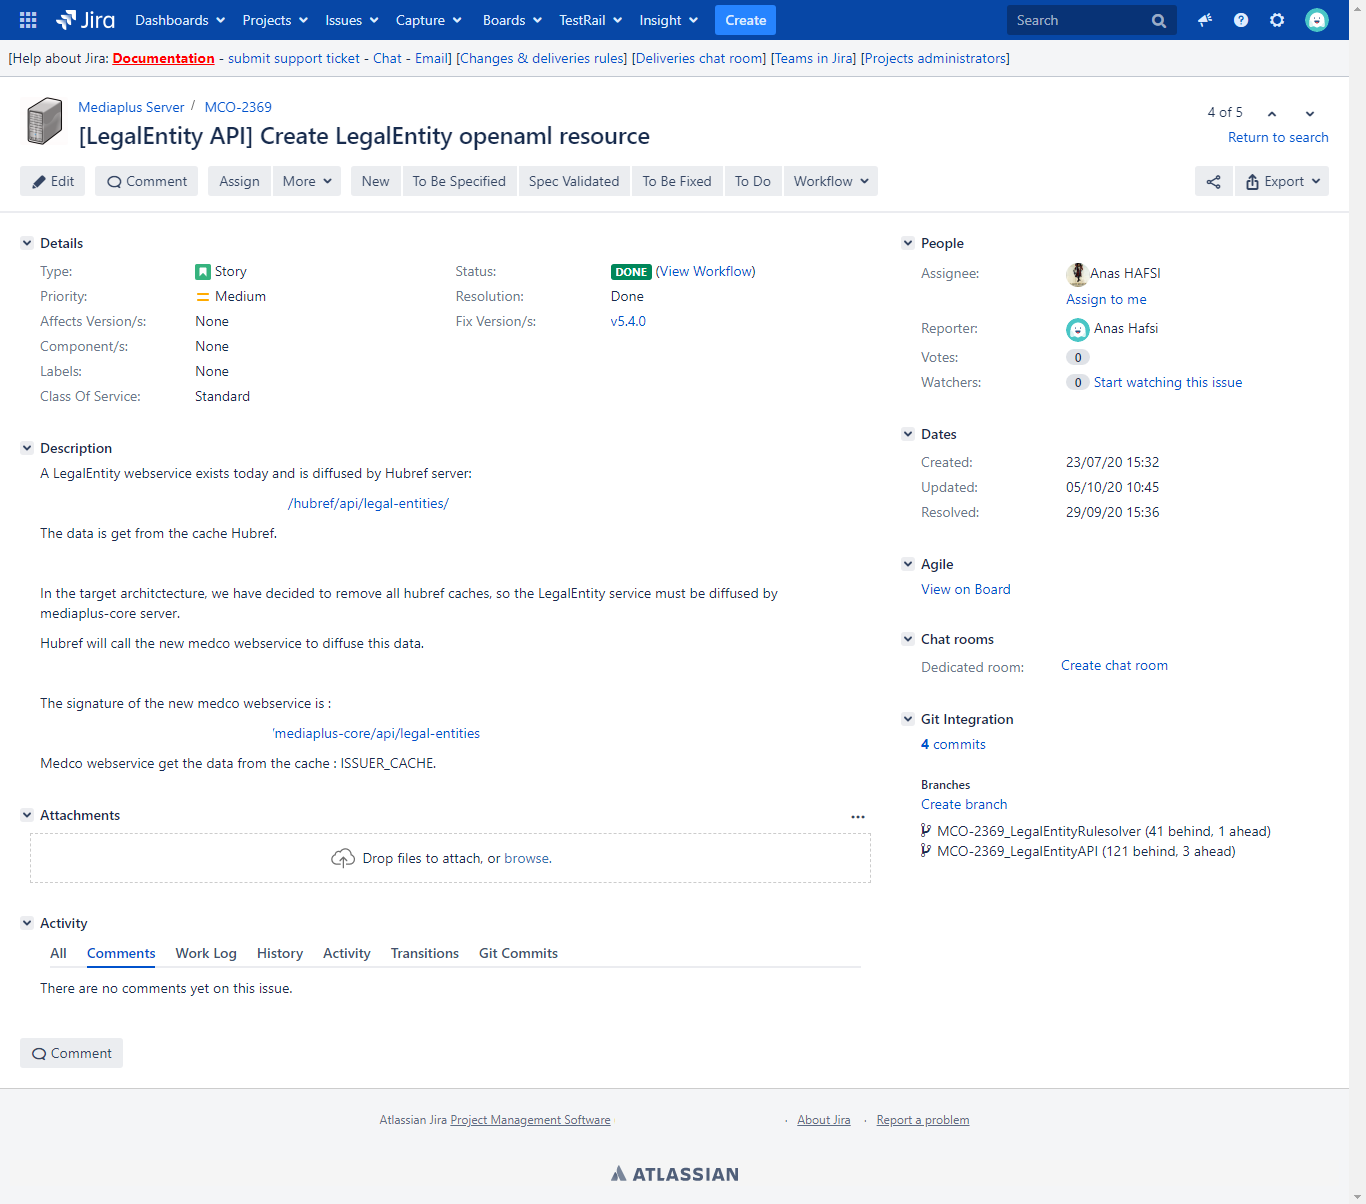
\includegraphics[width=\columnwidth]{img/JIRA MCO-2369.png}
    \caption{Ticket Jira MediaPlus Core}
    \label{fig:JiraMedco}
\end{figure}

\par Les "Issue" Jira sont nommée des tickets (exemple figure \ref{fig:JiraMedco}). l'ensemble de tickets appartenant au même sprint Agile sont rassemblé dans un "board JIRA" (exemple figure \ref{fig:JiraAlto}).
\clearpage
\begin{figure}[ht]
    \centering
    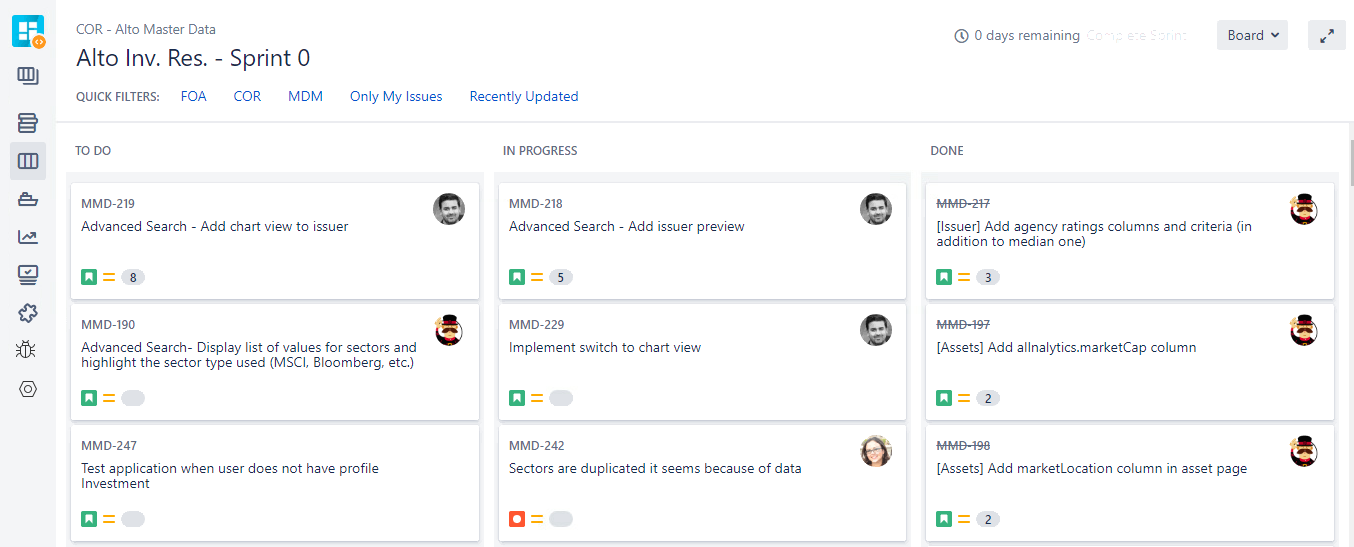
\includegraphics[width=\columnwidth]{img/Sprint Alto.png}
    \caption{Jira Board pour un sprint Alto Investment Research}
    \label{fig:JiraAlto}
\end{figure}
\subsubsection{Confluence}
\par Créez, collaborez et organisez tout votre travail à un seul et même endroit. Confluence est un espace de travail en équipe où la connaissance et la collaboration se rejoignent. Les pages dynamiques permettent à votre équipe de disposer d'un endroit pour créer, capturer et collaborer sur le projet ou l'idée de votre choix. Grâce aux espaces, votre équipe peut structurer, organiser et partager les tâches, afin que chacun de ses membres dispose d'une visibilité sur les connaissances institutionnelles ainsi que d'un accès aux informations nécessaires pour optimiser le travail.
\par Confluence s'adresse aux équipes de toute taille et de tout type. Qu'il s'agisse d'équipes ayant des projets stratégiques aux enjeux élevés, qui nécessitent de la rigueur dans leurs pratiques, ou d'équipes à la recherche d'un espace pour développer une culture d'équipe et interagir les unes avec les autres de manière plus ouverte et plus authentique. Grâce à Confluence, votre équipe peut prendre des décisions rapides, gagner en alignement et accomplir plus ensemble. {\tiny source: Atlassian documentation}
\par La figure \ref{fig:conf} represente un espace confluence.
\begin{figure}[ht]
    \centering
    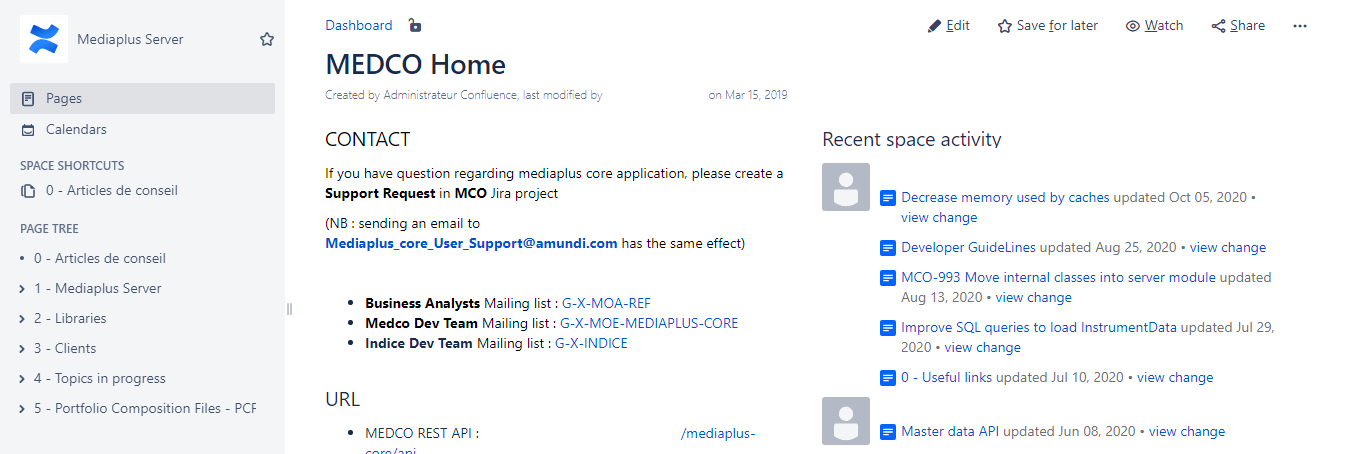
\includegraphics[width=\columnwidth]{img/ConfMedco.png}
    \caption{Espace Confluence MediaPlus-Core}
    \label{fig:conf}
\end{figure}

\subsection{Gitlab} 
\par GitLab est une plateforme de développement collaborative qui couvre l’ensemble des étapes du DevOps. Se basant sur les fonctionnalités du logiciel Git, elle permet de réaliser des dépôts et de gérer les versions de vos codes sources. Son usage est particulièrement indiqué pour les développeurs qui souhaitent disposer d’un outil réactif et accessible.
\par Comparé au autres logiciels de gestion de version, GitLab propose des options pour le moins pratiques :
\begin{itemize}
    \item Test de logiciels
    \item Configuration
    \item Monitoring
    \item Sécurité applicative
    \item Intégration et déploiement continus, etc\dots
\end{itemize}
\par Pour accompagner Gitlab on utilise SourceTree, un logiciel propriétaire du groupe Atlassian. C'est un logiciel front permettant de plus visualiser les branches git : un client frontend pour GitLab.
\begin{figure}[ht]
    \centering
    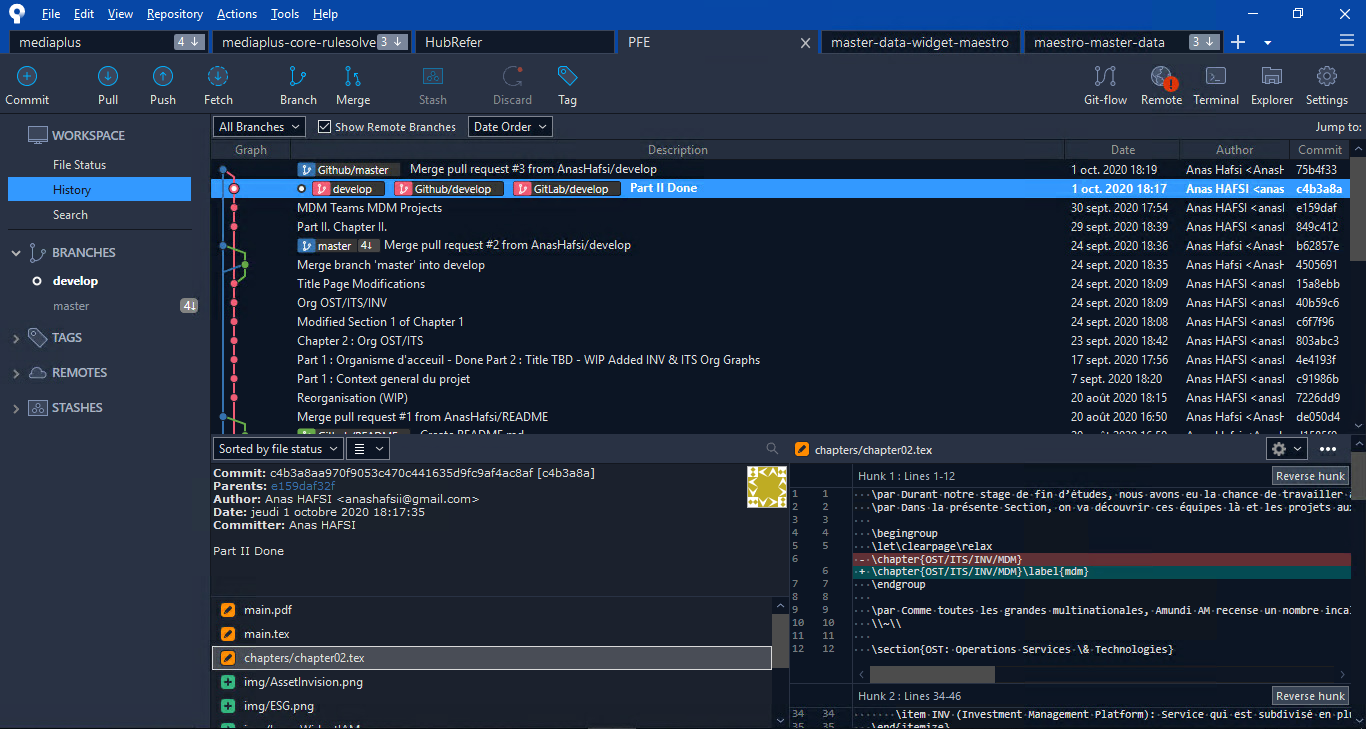
\includegraphics[width=\columnwidth]{img/sourcetree.png}
    \caption{SourceTree: interface pour la branche git contenant mon Rapport de stage}
\end{figure}
\clearpage
\subsection{Jenkins}
\par Jenkins est outil de compilation en continu des sources sur le serveur distant  Git. Il permet le lancement de processus automatiques : Compilation à  récurrence fixe, affichage de la dégradation de la qualité du code, lance les  tests unitaires des projets. Cet outil nécessite énormément de configuration  pour pour commencer à être productif. 
\par Jenkins contient une série de jobs génériques qui ont une utilité particulière. Il  nous est impossible de créer nos propres jobs génériques faute de droits (en  général de besoin. Les jobs génériques couvrent quasiment tous les cas)
\begin{figure}[ht]
    \centering
    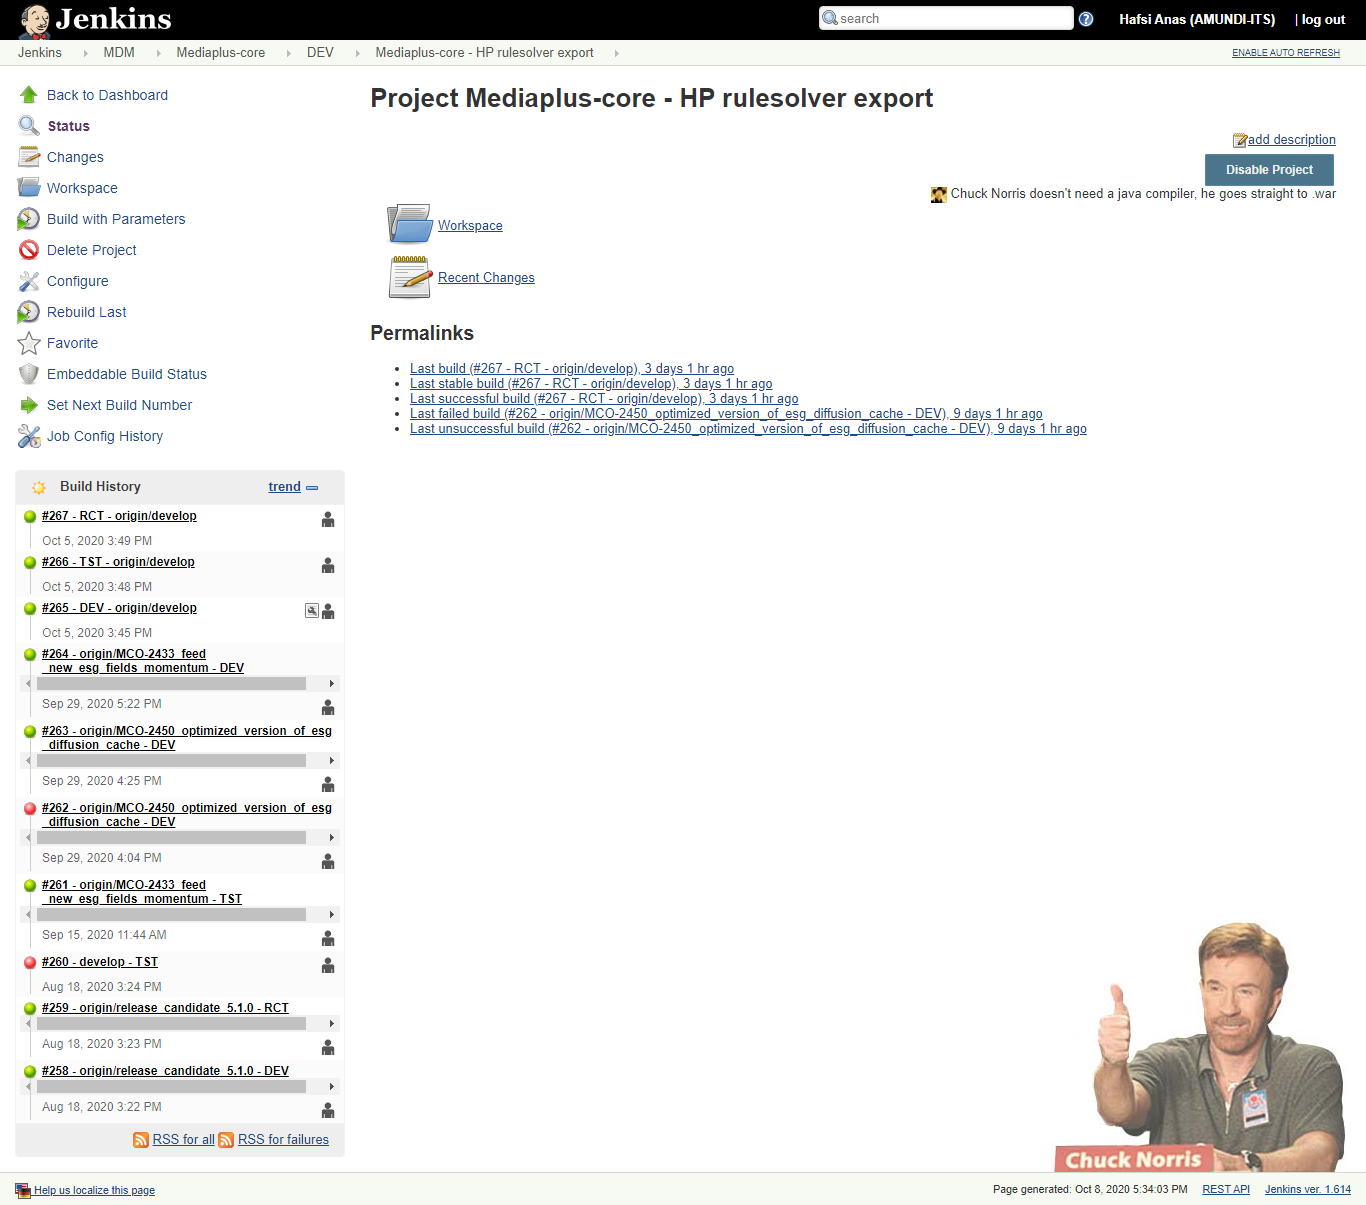
\includegraphics[width=\columnwidth]{img/jenkins.png}
    \caption{Interface Jenkins pour une branche MediaPlus-Core}
\end{figure}
\section{Outils MediaPlus Core}
\section{Outils Alto Investment Research}